\section{Visual comparison for all four backbones}
\label{sec:supp_subjective}

Fig.~\ref{fig:supp_subjective} repeats the visual comparison of the main paper for all four
backbones at full resolution. The layout is the same. Every cell is a zoomed region chosen
automatically as the window inside tissue where the wrapper changed the NAFNet output most, because
a change too small to see at full scale is the normal case and the reader should be shown the
largest one rather than an average one. The last column
shows the change the wrapper applied, on a scale symmetric about zero, so the reader can see where
the correction acted rather than inferring it.

\begin{figure*}[t]
\centering
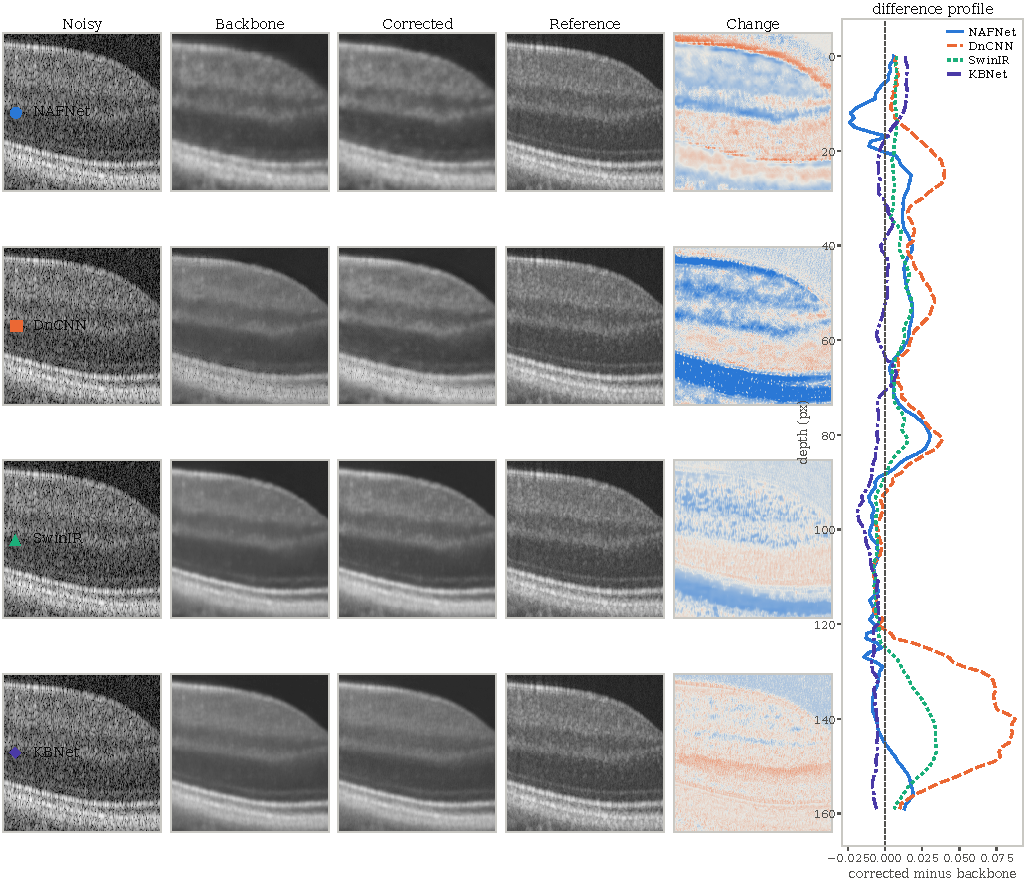
\includegraphics[width=\textwidth]{figures/fig_subjective_all.pdf}
\caption{Visual comparison on PKU37 for all four backbones. Columns are the noisy input, the backbone
output, the corrected output, the clean reference, and the change applied. Orange means the wrapper
lowered the value and blue means it raised it. The rightmost panel is the difference profile across
depth for all four backbones over the same crop.}
\label{fig:supp_subjective}
\end{figure*}
